\documentclass[11pt,a4paper]{article}

% Packages
\usepackage[margin=2.5cm]{geometry}
\usepackage{microtype}
\usepackage{graphicx}
\usepackage{tikz}
\usetikzlibrary{shapes,arrows.meta,positioning,calc,fit,backgrounds,shadows.blur,decorations.pathmorphing,decorations.pathreplacing}
\usepackage{colortbl}
\usepackage{enumitem}
\usepackage{booktabs}
\usepackage{longtable}
\usepackage{hyperref}
\usepackage{xcolor}
\usepackage{fancyhdr}
\usepackage{titlesec}
\usepackage[most]{tcolorbox}
\usepackage{multicol}
\usepackage{amsmath,amssymb}
\usepackage{multirow}
\usepackage{setspace}
\usepackage{fontawesome5}
\usepackage{listings}

% Spacing
\setlength{\parskip}{3pt plus 1pt minus 1pt}
\setlength{\parindent}{0pt}

% Colors
\definecolor{primary}{HTML}{0E4D64}
\definecolor{secondary}{HTML}{137177}
\definecolor{accent}{HTML}{C84B31}
\definecolor{lightbg}{HTML}{E8F6F3}
\definecolor{defbg}{HTML}{FDF2E9}
\definecolor{greenhl}{HTML}{2E8B57}
\definecolor{purplehl}{HTML}{6C5B7B}
\definecolor{codebg}{HTML}{F4F6F7}

% Hyperref
\hypersetup{colorlinks=true, linkcolor=primary, urlcolor=secondary, citecolor=primary}

% Code/listing style
\lstset{
  backgroundcolor=\color{codebg},
  basicstyle=\ttfamily\small,
  keywordstyle=\color{primary}\bfseries,
  stringstyle=\color{greenhl},
  commentstyle=\color{gray},
  breaklines=true,
  frame=l,
  framerule=2pt,
  rulecolor=\color{secondary!40},
  xleftmargin=8pt,
  framexleftmargin=6pt,
  aboveskip=6pt,
  belowskip=6pt
}

% Header/Footer
\pagestyle{fancy}
\fancyhf{}
\fancyhead[L]{\small\textcolor{primary}{\textbf{Mathematical Foundations of Data Science --- BSIT}}}
\fancyhead[R]{\small\textcolor{primary}{Lecture Handout}}
\fancyfoot[C]{\small\thepage}
\renewcommand{\headrulewidth}{0.5pt}
\renewcommand{\footrulewidth}{0.3pt}

% Section formatting
\titleformat{\section}{\Large\bfseries\color{primary}}{\thesection}{0.6em}{}[\vspace{2pt}\titlerule]
\titleformat{\subsection}{\large\bfseries\color{secondary}}{\thesubsection}{0.5em}{}
\titleformat{\subsubsection}{\normalsize\bfseries\color{primary}}{\thesubsubsection}{0.5em}{}
\titlespacing*{\section}{0pt}{14pt}{8pt}
\titlespacing*{\subsection}{0pt}{10pt}{5pt}

% Custom boxes
\newtcolorbox{definitionbox}[1][] {
  enhanced, breakable,
  colback=defbg, colframe=orange!60!black,
  colbacktitle=orange!70!black, coltitle=white,
  title={\faIcon{book}~#1}, fonttitle=\bfseries,
  boxrule=0pt, leftrule=4pt, arc=2pt,
  shadow={1mm}{-1mm}{0mm}{black!15},
  top=4pt, bottom=4pt, left=8pt, right=8pt
}
\newtcolorbox{conceptbox}[1][] {
  enhanced, breakable,
  colback=lightbg, colframe=secondary,
  colbacktitle=secondary, coltitle=white,
  title={\faIcon{lightbulb}~#1}, fonttitle=\bfseries,
  boxrule=0pt, leftrule=4pt, arc=2pt,
  shadow={1mm}{-1mm}{0mm}{black!15},
  top=4pt, bottom=4pt, left=8pt, right=8pt
}
\newtcolorbox{alertbox}[1][] {
  enhanced, breakable,
  colback=red!4, colframe=accent,
  colbacktitle=accent, coltitle=white,
  title={\faIcon{exclamation-triangle}~#1}, fonttitle=\bfseries,
  boxrule=0pt, leftrule=4pt, arc=2pt,
  shadow={1mm}{-1mm}{0mm}{black!12},
  top=3pt, bottom=3pt, left=8pt, right=8pt
}
\newtcolorbox{examplebox}[1][] {
  enhanced, breakable,
  colback=green!4, colframe=greenhl,
  colbacktitle=greenhl, coltitle=white,
  title={\faIcon{code}~#1}, fonttitle=\bfseries,
  boxrule=0pt, leftrule=4pt, arc=2pt,
  shadow={1mm}{-1mm}{0mm}{black!12},
  top=3pt, bottom=3pt, left=8pt, right=8pt
}

\begin{document}

% Title
\begin{center}
\vspace*{0.5cm}
{\Huge\bfseries\textcolor{primary}{Mathematical Foundations of Data Science}}\\[8pt]
{\Large\bfseries\textcolor{primary}{Concepts, Intuition, and Simple Calculations}}\\[16pt]
{\color{secondary}\rule{0.74\textwidth}{1.5pt}}\\[12pt]
{\Large\textsc{BSIT Lecture Handout}}\\[6pt]
{\large\textcolor{gray!70!black}{Course: Data Science \quad Program: BSIT}}\\[8pt]
{\normalsize\textcolor{gray!70!black}{Numbers \textbullet\ Vectors \textbullet\ Probability \textbullet\ Statistics \textbullet\ Optimization}}
\vspace{0.3cm}
\end{center}

\tableofcontents
\newpage

%=============================================================
\section{Why Mathematics Matters in Data Science}
%=============================================================

\begin{definitionbox}[Mathematical Foundations]
Mathematical foundations of data science are the core ideas from arithmetic, algebra, linear algebra, probability, statistics, and calculus that help us describe data, build models, measure uncertainty, and optimize predictions.
\end{definitionbox}

\begin{conceptbox}[Big Picture]
Data science is not only about coding tools. Every chart, model, prediction, and evaluation metric rests on mathematical reasoning. Mathematics helps answer questions such as: How large is the average? How uncertain is a prediction? How similar are two records? How does a model improve step by step?
\end{conceptbox}

\subsection{What Mathematics Helps Us Do}

\begin{itemize}[leftmargin=*]
  \item Summarize datasets using averages and spread.
  \item Represent data in vectors and matrices.
  \item Measure uncertainty using probability.
  \item Find relationships using correlation and covariance.
  \item Minimize errors using optimization.
\end{itemize}

\subsection{A Quick Roadmap}

\begin{longtable}{p{3.2cm}p{8.2cm}}
\toprule
\textbf{Math Area} & \textbf{Common Data Science Use} \\
\midrule
Algebra & Writing formulas for models and metrics \\
Linear algebra & Storing features and performing transformations \\
Probability & Modeling uncertainty and event likelihood \\
Statistics & Summarizing, comparing, and interpreting data \\
Calculus & Improving models by minimizing loss functions \\
\bottomrule
\end{longtable}

%=============================================================
\section{Numbers, Algebra, and Functions}
%=============================================================

\subsection{Basic Arithmetic in Data Science}

Data science often begins with basic operations:

\begin{itemize}[leftmargin=*]
  \item Addition and subtraction for totals and changes.
  \item Multiplication and division for rates and averages.
  \item Ratios and percentages for comparison.
\end{itemize}

\begin{examplebox}[Percentage Example]
Suppose 18 out of 24 students passed a quiz. The pass rate is
\[
\text{Pass rate} = \frac{18}{24} \times 100 = 75\%
\]
This simple percentage is already a useful data summary.
\end{examplebox}

\subsection{Variables and Simple Formulas}

In mathematics, a variable is a symbol that represents a value. For example, if $x$ is the number of hours studied, then a very simple score model might be
\[
y = 5x + 40
\]
If a student studies for $x = 6$ hours, then
\[
y = 5(6) + 40 = 70
\]

\subsection{Functions}

A function maps an input to an output.

\begin{definitionbox}[Function]
A function is a rule that takes one or more inputs and produces an output. In data science, models are functions that transform input features into predictions.
\end{definitionbox}

\begin{center}
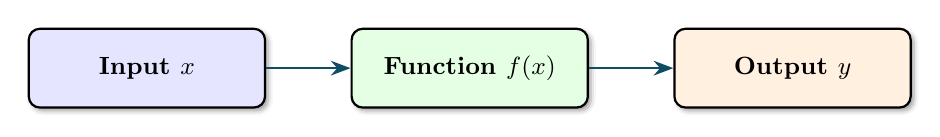
\begin{tikzpicture}[
  nodebox/.style={rectangle, draw, thick, rounded corners=4pt, minimum width=3cm, minimum height=1cm, align=center, font=\small\bfseries,
    blur shadow={shadow blur steps=3, shadow xshift=0.4mm, shadow yshift=-0.4mm}},
  arr/.style={-{Stealth[length=2.5mm]}, thick, primary}
]
  \node[nodebox, fill=blue!10] (input) at (0,0) {Input $x$};
  \node[nodebox, fill=green!10] (func) at (4.1,0) {Function $f(x)$};
  \node[nodebox, fill=orange!12] (output) at (8.2,0) {Output $y$};
  \draw[arr] (input) -- (func);
  \draw[arr] (func) -- (output);
\end{tikzpicture}
\end{center}

\subsection{Common Function Shapes}

\begin{itemize}[leftmargin=*]
  \item \textbf{Linear:} $y = mx + b$
  \item \textbf{Quadratic:} $y = ax^2 + bx + c$
  \item \textbf{Exponential:} $y = ab^x$
  \item \textbf{Sigmoid:} $\sigma(z) = \frac{1}{1 + e^{-z}}$
\end{itemize}

\begin{conceptbox}[Why Functions Matter]
Regression, classification, recommendation systems, and neural networks all rely on functions. The main difference is how simple or complex the function is.
\end{conceptbox}

%=============================================================
\section{Vectors and Matrices}
%=============================================================

\subsection{Vectors}

A vector is an ordered list of numbers. In data science, one row of features can be represented as a vector.

\[
\mathbf{x} = \begin{bmatrix} 2 \\ 4 \\ 6 \end{bmatrix}
\]

If the values represent \emph{hours studied}, \emph{assignments completed}, and \emph{attendance score}, then the vector stores one student's features.

\begin{examplebox}[Vector Addition]
Let
\[
\mathbf{a} = \begin{bmatrix} 1 \\ 2 \end{bmatrix}, \qquad
\mathbf{b} = \begin{bmatrix} 3 \\ 5 \end{bmatrix}
\]
Then
\[
\mathbf{a} + \mathbf{b} = \begin{bmatrix} 1+3 \\ 2+5 \end{bmatrix} = \begin{bmatrix} 4 \\ 7 \end{bmatrix}
\]
\end{examplebox}

\subsection{Dot Product}

The dot product combines two vectors into one number:
\[
\mathbf{a} \cdot \mathbf{b} = a_1b_1 + a_2b_2 + \cdots + a_nb_n
\]

\begin{examplebox}[Dot Product Calculation]
Let
\[
\mathbf{a} = \begin{bmatrix} 2 \\ 3 \end{bmatrix}, \qquad
\mathbf{b} = \begin{bmatrix} 4 \\ 5 \end{bmatrix}
\]
Then
\[
\mathbf{a} \cdot \mathbf{b} = (2)(4) + (3)(5) = 8 + 15 = 23
\]
The dot product is important in linear models and similarity calculations.
\end{examplebox}

\subsection{Matrices}

A matrix is a rectangular table of numbers. Datasets are often stored as matrices.

\[
X = \begin{bmatrix}
1 & 2 & 80 \\
2 & 4 & 75 \\
3 & 5 & 92
\end{bmatrix}
\]

Each row can represent one observation, and each column can represent one feature.

\begin{conceptbox}[Matrix Interpretation]
If a dataset has $m$ rows and $n$ columns, then it can be seen as an $m \times n$ matrix. Many machine learning algorithms operate directly on this structure.
\end{conceptbox}

\subsection{Distance Between Two Points}

For two points $(x_1, y_1)$ and $(x_2, y_2)$, Euclidean distance is
\[
d = \sqrt{(x_2 - x_1)^2 + (y_2 - y_1)^2}
\]

\begin{examplebox}[Distance Example]
Find the distance between $(1,2)$ and $(4,6)$:
\[
d = \sqrt{(4-1)^2 + (6-2)^2} = \sqrt{3^2 + 4^2} = \sqrt{9 + 16} = \sqrt{25} = 5
\]
Distance is used in clustering and nearest-neighbor methods.
\end{examplebox}

%=============================================================
\section{Statistics for Describing Data}
%=============================================================

\subsection{Mean, Median, and Mode}

Suppose the quiz scores are: $60, 70, 70, 80, 90$

\begin{itemize}[leftmargin=*]
  \item \textbf{Mean:} average value
  \item \textbf{Median:} middle value after sorting
  \item \textbf{Mode:} most frequent value
\end{itemize}

\begin{examplebox}[Mean, Median, Mode]
For the scores $60, 70, 70, 80, 90$:
\[
\text{Mean} = \frac{60 + 70 + 70 + 80 + 90}{5} = \frac{370}{5} = 74
\]
Sorted data is already $60, 70, 70, 80, 90$, so
\[
\text{Median} = 70
\]
The most frequent value is also
\[
\text{Mode} = 70
\]
\end{examplebox}

\subsection{Range, Variance, and Standard Deviation}

\begin{itemize}[leftmargin=*]
  \item \textbf{Range:} maximum minus minimum
  \item \textbf{Variance:} average squared distance from the mean
  \item \textbf{Standard deviation:} square root of the variance
\end{itemize}

\begin{examplebox}[Variance and Standard Deviation]
Consider the data: $2, 4, 6$

Step 1: Find the mean.
\[
\bar{x} = \frac{2 + 4 + 6}{3} = 4
\]

Step 2: Find deviations from the mean.
\[
2 - 4 = -2, \qquad 4 - 4 = 0, \qquad 6 - 4 = 2
\]

Step 3: Square the deviations.
\[
(-2)^2 = 4, \qquad 0^2 = 0, \qquad 2^2 = 4
\]

Step 4: Average the squared deviations.
\[
\text{Variance} = \frac{4 + 0 + 4}{3} = \frac{8}{3} \approx 2.67
\]

Step 5: Take the square root.
\[
\text{Standard deviation} = \sqrt{\frac{8}{3}} \approx 1.63
\]
\end{examplebox}

\subsection{Why Spread Matters}

Two datasets can have the same mean but different variability. In practice, a low-spread dataset is more consistent, while a high-spread dataset is more scattered.

\begin{alertbox}[Practical Warning]
An average alone can be misleading. If two classes both have mean score 75, but one class has very large spread, then performance consistency is quite different.
\end{alertbox}

\subsection{Z-Score}

A z-score shows how far a value is from the mean in standard deviation units:
\[
z = \frac{x - \bar{x}}{s}
\]

\begin{examplebox}[Z-Score Example]
Suppose a student score is $x = 85$, the class mean is $\bar{x} = 75$, and the standard deviation is $s = 5$.
\[
z = \frac{85 - 75}{5} = 2
\]
This means the score is 2 standard deviations above the mean.
\end{examplebox}

%=============================================================
\section{Probability and Uncertainty}
%=============================================================

\subsection{Basic Probability}

Probability measures how likely an event is.
\[
P(A) = \frac{\text{Number of favorable outcomes}}{\text{Total number of outcomes}}
\]

\begin{examplebox}[Simple Probability Example]
If a bag contains 3 red balls and 2 blue balls, then the probability of selecting a red ball is
\[
P(\text{red}) = \frac{3}{5} = 0.6
\]
So there is a 60\% chance of selecting red.
\end{examplebox}

\subsection{Conditional Probability}

Conditional probability asks for the probability of one event given that another event has already happened.
\[
P(A \mid B) = \frac{P(A \cap B)}{P(B)}
\]

\begin{examplebox}[Conditional Probability Example]
Suppose 20 students are in a class. 12 are male, and 5 are male and play basketball. Then the probability that a randomly chosen student plays basketball given that the student is male is
\[
P(\text{basketball} \mid \text{male}) = \frac{5}{12}
\]
\end{examplebox}

\subsection{Bayes' Idea}

Bayes' theorem updates probability when new evidence arrives:
\[
P(A \mid B) = \frac{P(B \mid A)P(A)}{P(B)}
\]

\begin{conceptbox}[Why Bayes Matters]
Spam detection, medical diagnosis, fraud detection, and classification all use the idea of updating beliefs when evidence is observed.
\end{conceptbox}

\subsection{Expected Value}

Expected value is the long-run average outcome:
\[
E(X) = \sum xP(x)
\]

\begin{examplebox}[Expected Value Example]
Suppose a simple game pays 10 pesos with probability 0.3 and 0 pesos with probability 0.7.
\[
E(X) = 10(0.3) + 0(0.7) = 3
\]
The expected value is 3 pesos.
\end{examplebox}

%=============================================================
\section{Covariance, Correlation, and Relationships}
%=============================================================

\subsection{Covariance}

Covariance tells us whether two variables tend to move together.

\begin{itemize}[leftmargin=*]
  \item Positive covariance: both increase together.
  \item Negative covariance: one increases while the other decreases.
  \item Near zero covariance: weak linear movement together.
\end{itemize}

\subsection{Correlation}

Correlation standardizes covariance so that the result lies between $-1$ and $1$.

\begin{itemize}[leftmargin=*]
  \item $r = 1$: perfect positive linear relationship
  \item $r = -1$: perfect negative linear relationship
  \item $r = 0$: no linear relationship
\end{itemize}

\begin{examplebox}[Interpreting Correlation]
If study hours and exam score have correlation $r = 0.82$, that suggests a strong positive linear relationship. As study hours increase, scores also tend to increase.
\end{examplebox}

\begin{alertbox}[Important Caution]
Correlation does not prove causation. Two variables can move together without one directly causing the other.
\end{alertbox}

%=============================================================
\section{Calculus and Optimization Intuition}
%=============================================================

\subsection{Slope and Derivative}

The derivative tells us how fast a quantity changes.

\begin{definitionbox}[Derivative]
The derivative measures the rate of change of a function. In machine learning, derivatives help determine how to adjust parameters to reduce error.
\end{definitionbox}

For example, if
\[
f(x) = x^2
\]
then
\[
f'(x) = 2x
\]

\begin{examplebox}[Simple Derivative Example]
For $f(x) = x^2$, find the slope at $x = 3$:
\[
f'(x) = 2x
\]
So at $x = 3$,
\[
f'(3) = 2(3) = 6
\]
This means the curve is increasing with slope 6 at that point.
\end{examplebox}

\subsection{Loss Function}

A loss function measures prediction error. One common example is mean squared error:
\[
\text{MSE} = \frac{1}{n}\sum_{i=1}^{n}(y_i - \hat{y}_i)^2
\]

\begin{examplebox}[MSE Calculation]
Suppose actual values are $[4, 6]$ and predicted values are $[5, 5]$.
\[
\text{MSE} = \frac{(4-5)^2 + (6-5)^2}{2} = \frac{1 + 1}{2} = 1
\]
The average squared error is 1.
\end{examplebox}

\subsection{Gradient Descent Intuition}

Gradient descent is a step-by-step method for reducing error.

\begin{center}
\begin{tikzpicture}[
  scale=0.95,
  point/.style={circle, fill=accent, inner sep=1.6pt},
  arr/.style={-{Stealth[length=2.5mm]}, thick, accent}
]
  \draw[->, thick] (-0.2,0) -- (6.3,0) node[right] {$x$};
  \draw[->, thick] (0,-0.2) -- (0,4.8) node[above] {Loss};
  \draw[domain=0.4:5.8, smooth, variable=\x, primary, thick] plot ({\x},{0.45*(\x-3)^2+0.6});
  \node[point] (p1) at (5.1,2.49) {};
  \node[point] (p2) at (4.3,1.28) {};
  \node[point] (p3) at (3.5,0.71) {};
  \node[point] (p4) at (3.0,0.60) {};
  \draw[arr] (p1) -- (p2);
  \draw[arr] (p2) -- (p3);
  \draw[arr] (p3) -- (p4);
\end{tikzpicture}
\end{center}

\begin{conceptbox}[Optimization Idea]
If a model makes large errors, gradient-based optimization changes the parameters in the direction that reduces the loss. This is one of the key ideas behind linear regression, logistic regression, and neural networks.
\end{conceptbox}

%=============================================================
\section{From Mathematics to Machine Learning Models}
%=============================================================

\subsection{Linear Regression Idea}

Linear regression predicts a numeric output using a straight-line equation:
\[
\hat{y} = b_0 + b_1x
\]

\begin{examplebox}[Linear Regression Example]
Suppose a model is
\[
\hat{y} = 40 + 5x
\]
If a student studies for $x = 7$ hours, then the predicted score is
\[
\hat{y} = 40 + 5(7) = 75
\]
\end{examplebox}

\subsection{Logistic Regression Idea}

Logistic regression predicts probabilities for two-class problems using the sigmoid function:
\[
\sigma(z) = \frac{1}{1 + e^{-z}}
\]

\begin{examplebox}[Probability Interpretation]
If a logistic model outputs $0.82$, that means the model estimates an 82\% probability that the observation belongs to the positive class.
\end{examplebox}

\subsection{Feature Scaling}

Features measured on very different scales can distort calculations.

\begin{examplebox}[Scaling Example]
Suppose one feature is \emph{age} with values around 20, and another is \emph{family income} with values around 50000. The income feature may dominate distance or gradient calculations. Standardization helps by putting features on comparable scales.
\end{examplebox}

%=============================================================
\section{Quick Reference Summary}
%=============================================================

\begin{longtable}{p{3.4cm}p{7.8cm}}
\toprule
\textbf{Concept} & \textbf{Key Formula or Idea} \\
\midrule
Mean & $\bar{x} = \frac{\sum x}{n}$ \\
Variance & Average squared distance from the mean \\
Standard deviation & Square root of variance \\
Probability & $P(A) = \frac{\text{favorable}}{\text{total}}$ \\
Distance & $d = \sqrt{\sum (x_i-y_i)^2}$ \\
Dot product & $\mathbf{a} \cdot \mathbf{b} = \sum a_ib_i$ \\
Derivative & Rate of change of a function \\
MSE & $\frac{1}{n}\sum (y_i - \hat{y}_i)^2$ \\
Correlation & Strength and direction of linear relationship \\
\bottomrule
\end{longtable}

%=============================================================
\section{Key Takeaways and Review Questions}
%=============================================================

\subsection{Key Takeaways}

\begin{itemize}[leftmargin=*]
  \item Data science relies on core mathematics, not just software tools.
  \item Algebra and functions help express models and predictions.
  \item Vectors and matrices organize data for machine learning.
  \item Statistics summarizes center and spread.
  \item Probability handles uncertainty and evidence.
  \item Calculus supports optimization and model improvement.
\end{itemize}

\subsection{Review Questions}

\begin{enumerate}[leftmargin=*]
  \item What is the difference between a mean and a median?
  \item How is a vector different from a matrix?
  \item Why is probability important in classification problems?
  \item What does a positive correlation mean?
  \item Why do machine learning algorithms use loss functions?
  \item What role does the derivative play in optimization?
\end{enumerate}

\begin{examplebox}[Short Reflection Task]
Choose a small dataset from your daily life, such as quiz scores, phone usage hours, or daily expenses. Compute the mean, range, and standard deviation. Then explain what those numbers reveal about the data.
\end{examplebox}

\vfill
\begin{center}
{\large\textcolor{primary}{\textbf{End of Handout}}}\\[4pt]
{\small\textcolor{gray!70!black}{Mathematical Foundations of Data Science --- BSIT Program}}
\end{center}

\end{document}